\textbf{COLUNI 2022 -- Questão 32}\par\medskip Analise a charge do cartunista goiano Jorge Braga.

% COLUNI-AUTO-FIGURES-BEGIN
\begin{figure}[htbp]
\centering
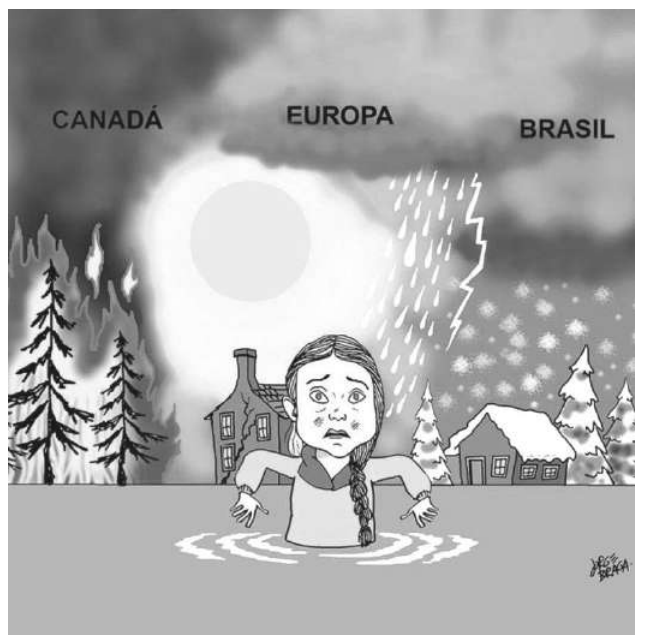
\includegraphics[width=0.95\linewidth]{static/simulados/coluni/figuras/2022/questao-32/figura-1.png}
\end{figure}
% COLUNI-AUTO-FIGURES-END

Disponível em: www.opopular.com.br. Acesso em: 29 jul. 2021.

\par

A charge representa uma intensificação do conjunto de fenômenos naturais que ocorreram no final de julho de 2021, em vários países e continentes. Levando-se em consideração que essa intensificação é uma representação do que vem ocorrendo no mundo, assinale a afirmativa CORRETA:


\begin{enumerate}
\item Está diretamente relacionada às características geológicas desses lugares, que possuem um relevo
      bastante elevado ou montanhoso, o que facilita as condições climáticas mais severas nessa estação do
      ano. Como exemplo, podemos citar a neve que caiu nas serras catarinenses.
\item A reduzida biodiversidade das paisagens nos locais citados contribui para a dinâmica atmosférica e para o
      intenso processo de desmatamento que vem ocorrendo de forma global. Observa-se uma significativa
      mudança nas condições climáticas, muitas vezes, resultando em tragédias.
\item As queimadas no Canadá, as enchentes na Europa e a neve no Brasil são resultantes da diversidade
      climática que esses locais possuem e isso ocorre em função da grande extensão territorial desses locais,
      que está diretamente relacionada ao fenômeno da continentalidade.
\item Nas últimas décadas, vem ocorrendo a intensificação dos fatores climáticos e ambientais que,
      influenciados pela ação antrópica, contribuem para o aquecimento global, provocando alterações na
      temperatura média do planeta e na dinâmica dos climas.\end{enumerate}
